\section{Theoretical Analysis}
\label{sec:analysis}

In this circuit, we have a multiple negative feedback applied via the equivalent resistor R2 and the
and the equivalent capacitor C2.

Moreover, the capcitor C2 blocks the input signals with low frequency and the capacitor C1
blocks the input signal with high frequencies.

\subsection{OP-AMP model}

In the theoretical part, we use the ideal model of the OP-AMP. So, we consider the input impedance equals to $\infty \Omega$, the ouput impedance
equals to $0 \Omega$, and the gain equal to $\infty$. As a consequence, the differences of voltage of the non inverting input $v_{+}$ and The
inverting input $_v{-}$ is equal to zero and we have a \textit{virtual ground} in the non inverting input.


\subsection{Frequency response}

In order to obtain, the transfer function, we use nodal analysis method to obtain the following system of equations:

\[
  \begin{bmatrix}
    \frac{1}{R_1} + \frac{1}{Z_{C1}} + \frac{1}{Z_{C2}} & -\frac{1}{Z_{C2}} \\
    -\frac{1}{Z_{C1}}                                   & -\frac{1}{R_2}    \\
  \end{bmatrix}
  \begin{bmatrix}
    V_{1} \\ V_{out}
  \end{bmatrix}
  \begin{bmatrix}
    \frac{V_{in}}{R_1} \\ 0
  \end{bmatrix}
\]

\hfill



\begin{equation}
  T(\omega) = \frac{\widetilde{V_{out}}}{\widetilde{V_{in}}}
  \label{frequencyR}
\end{equation}

We use Octave to solve this system of equations numerically for a differences range of frequencies of the input signal.

In plot \ref{fig:output1}, we have the phase, obtained by taking the $arg(T(\omega))$, as function of log (f) in Hz.

Input Impedance Output Impedance

\begin{figure*}[h]
  \centering
  \begin{subfigure}{0.5\textwidth}
    \includegraphics[width=\linewidth, clip]{phase.eps}
    \label{fig:output1}
  \end{subfigure}
  \begin{subfigure}{0.4\textwidth}
    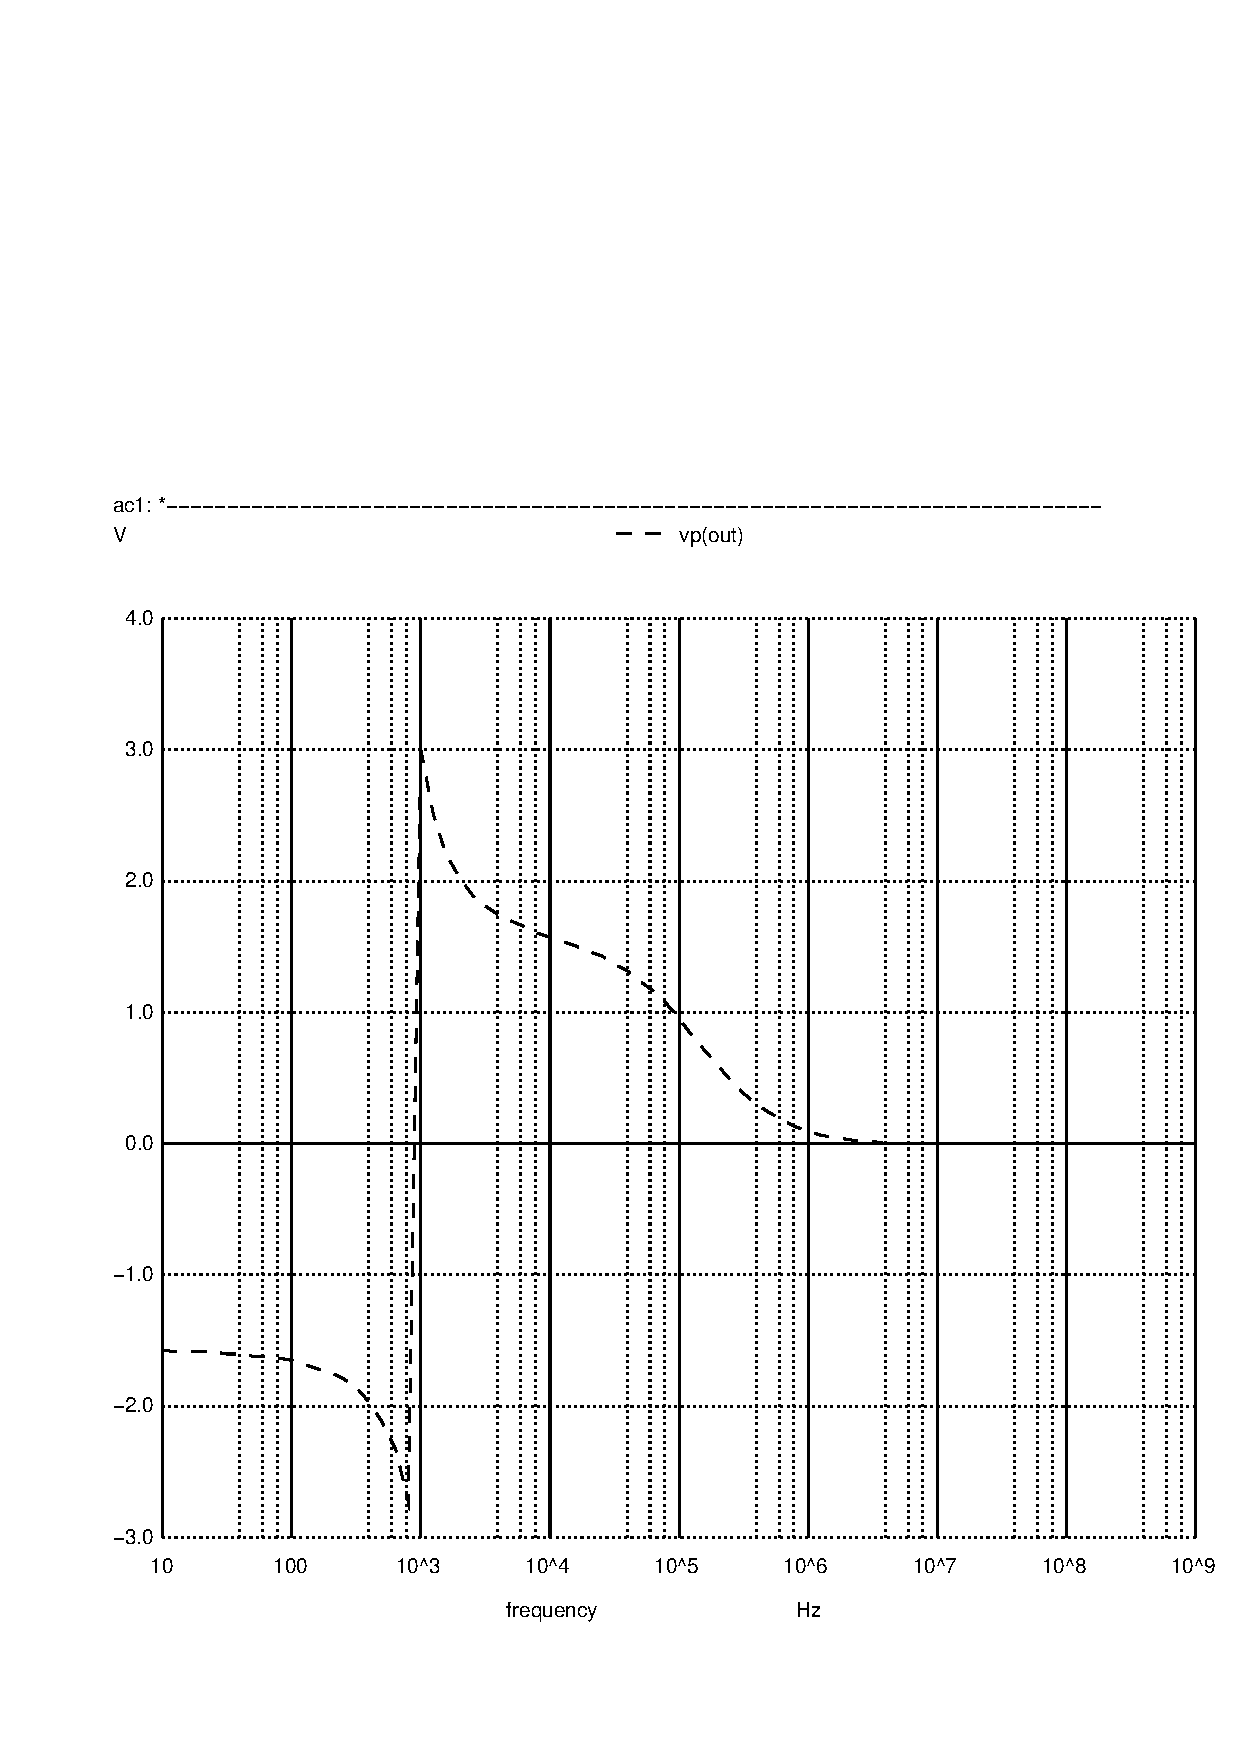
\includegraphics[width=\linewidth, clip]{phase.pdf}
    \label{fig:output2}
  \end{subfigure}
  \caption{\small  )}
  \label{output_deviation}
\end{figure*}


In plot \ref{fig:argTOct} we have the magnitude, calculated from $20*log_{10}(abs(T(\omega)))$ as function of log(f) .

\begin{figure*}[h]
  \centering
  \begin{subfigure}{0.5\textwidth}
    \includegraphics[width=\linewidth, clip]{gain.eps}
    \label{fig:argTOct}
  \end{subfigure}
  \begin{subfigure}{0.4\textwidth}
    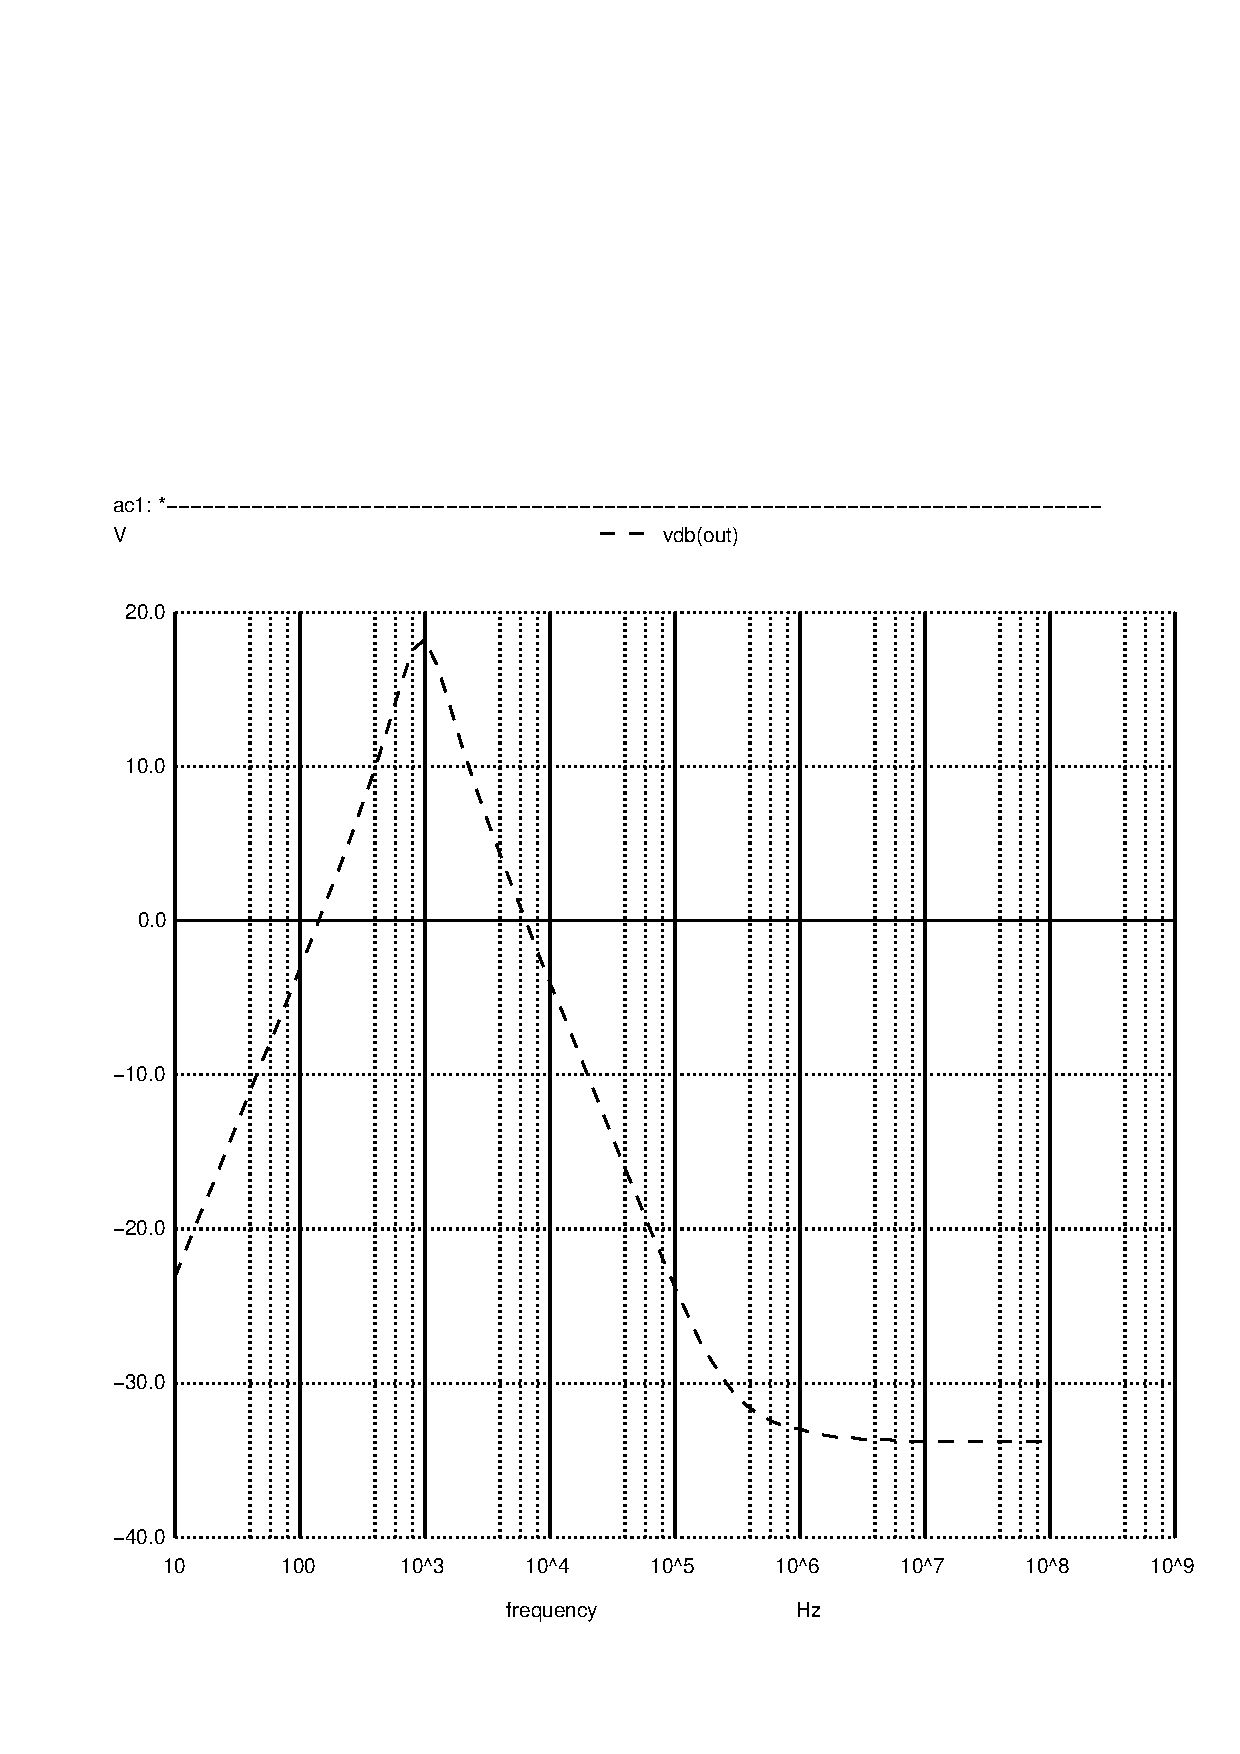
\includegraphics[width=\linewidth, clip]{gain.pdf}
    \label{fig:argTSpi}
  \end{subfigure}
  \caption{\small }
  \label{}
\end{figure*}

\subsection{Input and Output Impedance and Central Frequency}

To evaluate the frequency of the input signal whose gain is maximized, we applied the \textit{max} function of Octave to the array in which
we have the valus of the magnitude of the gain. The value we get is presented in the table \ref*{tab:TheoreticalResults}.

In order to calculate the input impedance of the circuit in central frequency,
we use the following formula with a frequency of the input signal we get before:

\begin{equation}
  Z_{input} = \frac{V_{in}}{\frac{V_{in} - V_1}{R_1}} \frac{1}{1000} k \Omega
\end{equation}

Due to the teoretical model used for the OP-AMP, we have an $Z_{output} = 0$.


\begin{table}[h]
  % \parbox{.45\linewidth}{
  {
    \centering
    \begin{tabular}{|c|c|c|}
      \hline
      $Z_{input}$ & -1.312927e-01\\ \hline
$Z_{output}$ & 0.000000e+00\\ \hline
Max $Gain_{dB}$ & 1.835867e+01\\ \hline
Central frequency [Hz] & 9.660509e+02\\ \hline

    \end{tabular}
    \label{tab:TheoreticalResults}
    \caption{ }
  }
\end{table}

